\documentclass[../main.tex]{subfiles}
\graphicspath{{\subfix{../figures/}}}
\begin{document}
Equipped with the necessary theory, the dynamics of the parallel QD system can now be simulated. The equation of motion for the system is the Lindblad equation, given by \cref{eq:lind}, for the reduced density operator of the two quantum dots. In Fock-Liouville space, this is equation given by \cref{eq:lindfock}, with a matrix representation of the Liouvillian, $L$. Specifying the values of the parameters of the system, $L$ can be constructed from the jump operators and the effective Hamiltonian in the Lindblad equation. By then searching for coalescing eigenvalues and eigenvectors of $L$ in the parameter space, EPs can be located, at which the dynamics obey \cref{eq:genmode}. Finally, \cref{eq:expec} can be used to simulate the transient current through the parallel QD system. The numerical calculations were done in \verb+Python+ using standard tools from the \verb+numpy+ and \verb+scipy+ packages. Furthermore, a piece of code which already implemented the PERLind approach for calculating the jump operators and the Liouvillian was used as a starting point for further calculations. Both the pre-existing code and the code developed during the work of the thesis can be found in Ref.~\cite{git}.
\section{Model}
In this thesis, a particular quantum dot system was studied, consisting of two quantum dots connected to two leads, both of them in thermal equilibrium. Similarly to the works in e.g. Refs.~\cite{doubledot,doubledot2}, the quantum dots are assumed to be coupled in parallel to the leads, meaning that the dots are coupled to the same lead on each side. For simplicity, the electrons are assumed to be spinless, which is a good approximation for a low bias voltage in the presence of a magnetic field. However, the bias voltage considered in this thesis is cannot be considered to be small, and hence we must rely on an assumption of the system only containing one spin species. Furthermore, it is assumed that there is no direct tunneling between the dots. However, we consider an interacting system, with a finite contribution from the Coulomb repulsion between the electrons in the case of double occupancy. A sketch of the model is given in \cref{fig:model}.
\begin{figure}[H] \centering
    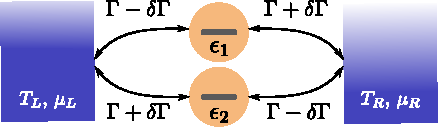
\includegraphics[width=0.8\linewidth]{figures/model.pdf}
    \caption{The modeled parallel dot system, where the quantum dots in the center have energies $\epsilon_1$ and $\epsilon_2$. Located on the sides are the two reservoirs $R,L$ with temperatures $T_{L/R}$ and chemical potentials $\mu_{L/R}$. The allowed tunneling processes are indicated with arrows, with corresponding tunneling rates $\Gamma \pm \delta\Gamma$.}
    \label{fig:model}
\end{figure}
To reduce the dimension of the parameter space, a fixed tunneling rate $\Gamma$ and a variable tunneling detuning $\delta\Gamma$ are introduced. The four tunneling rates in terms of $\Gamma$ and $\delta\Gamma$ are assumed to be asymmetric, as indicated by \cref{fig:model}. It is also assumed that each dot is restricted to be either empty or contain one (spinless) electron. The energy levels of the two QDs are assumed to given by $\epsilon_{1/2} = -V_\text{G} \pm \delta\epsilon$, with an energy detuning $\delta\epsilon$ and a gate voltage $V_\text{G}$, which we set to zero. Furthermore, the temperatures of the leads $T_\text{L}=T_\text{R}=10\Gamma$, the chemical potentials $\mu_\text{L/R} = \pm V_\text{SD}/2$, the bias voltage $V_\text{SD} = 300\Gamma$, and the Coulomb energy $U = 250\Gamma$, are all fixed in terms of $\Gamma$. This leaves the two tuning parameters, $\delta\Gamma$ and $\delta\epsilon$, as the only parameters of the system, resulting in a two dimensional parameter space. 

To be able to justify the Lindblad approach for calculating the dynamics of the system, one more major approximation has to be made regarding the coupling between the dots and the leads. We must assume that the strength of the coupling between the system and the environment is weak in comparison with the temperature, i.e., $\Gamma \ll T$. In this so called weak-coupling limit, the Lindblad equation is a standard approach for investigating the dynamics of a quantum dot system. In this thesis, we consider terms up to first order in  $\Gamma$. This approximation neglects effects such as cotunneling, where several electrons simultaneously tunnel into and out of the QDs. Hence, we only consider sequential tunneling processes.

The total system can be modeled by the Hamiltonian
\begin{equation}
    \hat H = \hat H_\text{QD} + \hat H_\text{leads} + \hat H_\text{tunneling},
\end{equation}
where the three terms correspond to the quantum dot, lead, and tunneling Hamiltonians
\begin{equation}
    \begin{split}
        \hat H_\text{QD} &= \sum_{i=1,2} \epsilon_i \hat d_i^\dag \hat d_i  + U\hat d_1^\dag \hat d_1 \hat d_2^\dag \hat d_2, \\
        \hat H_\text{leads} &= \sum_{k,s=\text{L,R}} E_{s, k} \hat c_{s,k}^\dag \hat c_{s,k}, \\
        \hat H_\text{tunneling} &= \sum_{i=1,2} \; \sum_{k,s=\text{L,R}} t_{s,i} \hat c_{s,k}^\dag \hat d_i + t_{s,i}^* \hat d_i^\dag \hat c_{s,k},
    \end{split}
\end{equation}
where $\hat d_i^\dag$ ($\hat d_i$), $i\in\{1,2\}$, creates (annihilates) an electron in dot 1 or 2, and $\hat c_{l,k}^\dag$~($\hat c_{l,k}$), $s\in\{\text{L,R}\}$, creates (annihilates) an electron in the left (L) or right (R) lead with momentum $k$ and energy $E_{s,k}$~\cite{doubledot}. The tunneling amplitudes $t_{s,i}$ are directly related to the corresponding tunneling rates by 
\begin{equation}
    \Gamma_{s,i} = 2\pi\nu_F|t_{s,i}|^2,
\end{equation}
where $\nu_F$ is the density of states in the lead, which we assume to be independent of energy~\cite{perlind}.

To represent the operators in matrix form, the many-body eigenstates of the isolated quantum dot Hamiltonian are used as the basis:
\begin{equation}\label{eq:basis}
    \begin{aligned}
        \ket{a} &= \ket{00} \\
        \ket{b} &= \ket{10} = \hat d_1^\dag\ket{00}\\
        \ket{c} &= \ket{01} = \hat d_2^\dag\ket{00}\\
        \ket{d} &= \ket{11} = \hat d_1^\dag\hat d_2^\dag\ket{00},\\
    \end{aligned}
\end{equation}
where $n_1$ and $n_2$ in $\ket{n_1n_2}$ are the number of electrons in the first and second QD, respectively. The quantum dot and tunneling Hamiltonians are in this basis given by
\begin{equation}
    \begin{aligned}
        \hat H_\text{QD} &= \epsilon_1\ket{b}\bra{b} + \epsilon_2\ket{c}\bra{c} + (\epsilon_1 + \epsilon_2 + U)\ket{d}\bra{d} \\
        \hat H_\text{tunneling} &= \sum_{k,s=\text{L,R}} \big[t_{s,1}^*(\ket{b}\bra{a} + \ket{d}\bra{c}) + t_{s,2}^*(\ket{c}\bra{a} - \ket{d}\bra{b})\big]\hat c_{s,k} + \text{H.c},
    \end{aligned}
\end{equation}
where the minus sign in the second term in the tunneling Hamiltonian comes from the fact that $d_2^\dag d_1^\dag = - d_1^\dag d_2^\dag$ for fermions.

In the basis given by \cref{eq:basis}, the elements of the reduced density matrix can be written as $\rho_{\alpha\beta}$, where $\alpha,\beta\in\{a,b,c,d\}$, with 16 matrix elements. However, the only non-zero off-diagonal elements are $\rho_{bc}$ and $\rho_{cb}$, i.e, the elements which corresponds to superpositions the two states with one occupied dot. This is the result of charge being a conserved quantity in the total system. The number of elements in $\ket{\rho}\rangle$ is therefore reduced to 6, which in turn means that the Liouvillian effectively can be represented by a $6\times6$ matrix. The vectorization of the density matrix can be done in several ways, but in this thesis it is given by
\begin{equation}\label{eq:order}
    \rho = \begin{bmatrix} \rho_{aa} & 0 & 0 & 0 \\
                    0 & \rho_{bb} & \rho_{bc} & 0 \\
                    0 & \rho_{cb} & \rho_{cc} & 0 \\
                    0 & 0 & 0 & \rho_{dd} \end{bmatrix} \rightarrow \ket{\rho}\rangle = \begin{bmatrix} \rho_{aa} \\ \rho_{bb} \\ \rho_{cc} \\ \rho_{dd} \\ \operatorname{Re}\rho_{bc} \\ \operatorname{Im}\rho_{bc}\end{bmatrix}.
\end{equation}
Since the density matrix is Hermitian, the diagonal elements are real and $\rho_{bc}=\rho_{cb}^*$. Hence, for the off-diagonal elements, it is enough to specify $\operatorname{Re}\rho_{bc}$ and $\operatorname{Im}\rho_{bc}$ to obtain an equivalent vectorized representation of the density matrix. The time evolution of the vectorized reduced density matrix is then determined by \cref{eq:lindfock}.


% The second main approximation is to assume that the interaction between the system and the environment is Markovian. A Markovian process is one in which the next time step only depends on the current state of the system. In a quantum dot system, this can be interpreted to mean that the leads "forget" that they have lost or gained an electron, right after the tunneling process has happened. Since the number of electrons in the leads typically is large, this can be a reasonable approximation for such systems.

\end{document}
